%! Author = hilfiker
%! Date = 21.07.2022

% Preamble
\documentclass[11pt]{article}

% Packages
\usepackage{amsmath} % Formulas in document
\usepackage{pdflscape} % Landscaped pages in Pdf
\usepackage[a4paper, margin=0.8in]{geometry} % Set the margin and size of a page
\usepackage[hidelinks]{hyperref} % Remove Boxes around Hyperlinks
\usepackage{lastpage} % Custom page numbering
\usepackage{fancyhdr}
\usepackage{graphicx}
\usepackage{mwe}
\usepackage{caption}
\usepackage{tcolorbox} % Custom page numbering

\usepackage{titling}
\usepackage{textcomp}
\usepackage{wasysym}
\usepackage[utf8]{inputenc}
\usepackage[T1]{fontenc}
\usepackage{enumerate}
\renewcommand\maketitlehooka{\null\mbox{}\vfill}
\renewcommand\maketitlehookd{\vfill\null}

\renewcommand*\contentsname{Inhaltsverzeichnis}
\renewcommand{\figurename}{Abb.}

% Configure page numbering & footer
\pagestyle{fancy}
\fancyhf{}
\lfoot{Tobias Hilfiker}
\cfoot{Seite \thepage \hspace{1pt} von \pageref{LastPage}}
\rfoot{\today}

% Methadata
\title{
    
\includegraphics[width=\textwidth]{media/curling_logo}
    \begin{center}
        Modul 152 \\
        Multimediainhalte in einen Webauftritt integrieren\\
        Storyboard
    \end{center}}
\author{Tobias Hilfiker}
\date{\today}

% Document
\begin{document}

    %Kapitel Frontpage
    \begin{titlingpage}
        \maketitle
    \end{titlingpage}
    \pagebreak

    %Kapitel Table of contents
    \tableofcontents
    \pagebreak

    %Kapitel 1 - Einleitung
    \section{Einleitung}
    Im Rahmen des Modul 152 darf ein E-Portfolio inklusive vorgehendem Storyboard erstellt werden.
    Dieses Storyboard soll eine Vorbereitung für das E-Portfolio sein, welches in einer separaten
    Dokumentation beschrieben wird.

    %Kapitel 1.1 - Ziel dieses Storyboards
    \subsection{Ziel dieses Storyboards}
    Mit diesem Storyboard habe ich das Ziel, die grundlegenden Konzepte für das E-Portfolio zu definieren.
    Dazu gehören Farbschemen, Logo, aber auch ein Mockup der Webseite.
    Folgende Fragen sollen bis zum Ende des Storyboards geklärt sein:
    \begin{itemize}
        \item Wie soll das Logo des E-Portfolios aussehen?
        \item Welche Farben sollen wo auf der Webseite verwendet werden? \textrightarrow Farbschema erstellen
        \item Wie soll die grundsätzliche Struktur des E-Portfolios aussehen?
        \textrightarrow Erstellung eines Mockups
        \item Welche Technologien möchte ich für die Erstellung der Webseite verwenden?
    \end{itemize}
    \\
    Neben den oben genannten Punkten möchte ich zudem bereits ein Bild, welches zum Thema passt bearbeiten.
    Um dieses Bild zu machen, informiere ich mich vorher in den Unterrichtsunterlagen und im Internet, welche
    Punkte beachtet werden müssen, um ein gutes Bild zu schiessen.
    Auch bei der Bildbearbeitung werde ich ähnlich vorgehen. Nachdem die Bildbearbeitung gelungen ist, werde
    ich eine Schritt-für-Schritt-Anleitung zu dieser Bildbearbeitungsmethode ins Storyboard schreiben.

    %Kapitel 1.2 - Spezielles
    \subsection{Spezielles}
    Um das Storyboard und die Dokumentation zum E-Portfolio zu schreiben, verwende ich \LaTeX. Das ist
    eine Skriptbasierte Dokumentationssprache, ähnlich wie Markdown. Primär gibt es zwei Unterschiede zu
    Markdown:
    \begin{enumerate}
        \item \LaTeX Dateien müssen kompiliert werden. Dazu gibt es verschiedene Compiler, welche aus den
        .tex-Dateien dann z.B.\ ein Pdf kompilieren.
        \item In ein \LaTeX Dokument können beliebig viele Packages eingebunden werden. Das bedeutet, dass
        Elemente wie Diagramme, oder eigene Formatierungen einfach in das gleiche Dokument eingebunden werden.
    \end{enumerate}

    \pagebreak
    %Kapitel 2 - Thema
    \section{Thema}

    Da wir freie Themenwahl hatten, habe ich mich für Curling entschieden.

    %Kapitel 2.1 - Wahl des Themas
    \subsection{Wahl des Themas}

    Ich habe das Thema Curling ausgewählt, da ich im Winter selbst Curling spiele. Dies tue ich bereits in der
    9. Saison in einem eingeschworenen Juniorenteam in St. Gallen.
    Meiner Meinung nach ist Curling eine sehr spannende Sportart, man muss beim Spielen sehr viele verschiedene
    Situationen abwägen, sich für die beste entscheiden und danach möglichst viele Faktoren zu seinen Gunsten
    beeinflussen. \\
    Die meisten Personen kennen Curling als Sportart und wirken auch meist sehr interessiert. Die meisten haben
    aber meist keine Ahnung von den Begriffen und den Regeln, was das Zuhören auf den Zuschauerbänken für mich
    meist sehr lustig gestaltet \smiley. Daher habe ich mit diesem E-Portfolio das Ziel, den Besuchern
    die Regeln und die Begrifflichkeiten etwas näher zu bringen.

    %Kapitel 3 - Visualisierung E-Portfolio
    \section{Visualisierung E-Portfolio}

    %Kapitel 3.1 - Menüstruktur
    \subsection{Menüstruktur}
    Als Menü-Navigation habe ich mich für eine Navigation am oberen Teil der Webseite entschieden. Dies ist
    auf den Mockups sehr gut ersichtlich. Darin ist das Logo und natürlich die Navigation in die verschiedenen
    Unterseiten enthalten.\\
    Auf Mobile habe ich mich dazu entschieden, das Menü mittels drei Linien immer im Header mit dem Logo
    eingeblendet zu haben. Tippt man auf die drei Linien öffnet sich ein Popup, welches dann das Menü anzeigt.

    \begin{figure}[h]
        \centering
        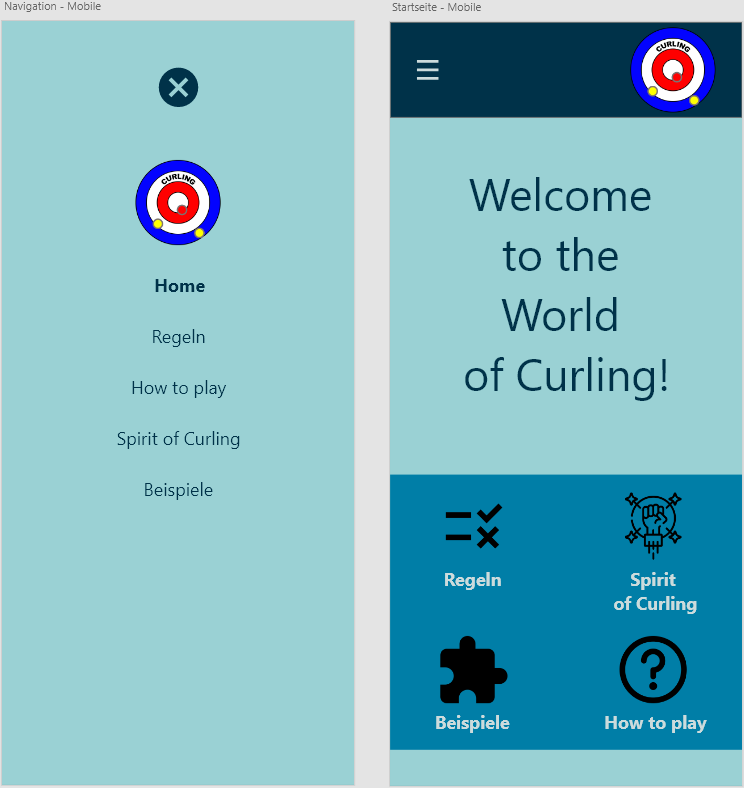
\includegraphics[height=11cm]{media/menu_mobile}
        \caption{Menü auf einem Mobilgerät}
    \end{figure}

    %Kapitel 3.2 - Farbwahl
    \subsection{Farbwahl}
    Um eine Farbauswahl habe ich mal simpel nach Farbpaletten im Internet gesucht. Dabei ist mir die Seite
    \url{colorhunt.co} aufgefallen. Diese Webseite lässt User ihre eigenen Farbpaletten hochladen und mit
    anderen Usern teilen. Zudem habe ich Adobe Color ausprobiert, allerdings ist dies viel zu viel
    Funktionalität für dieses Projekt. Daher werde ich für das Storyboard die Plattform Colorhunt verwenden.\\
    \\
    Auf Colorhunt selbst habe ich verschiedene Farbpaletten gefunden, welche ich im Folgenden aufgelistet
    habe. Gesucht habe ich nach Pastellfarbenen Farbpaletten gesucht, welche an Winter, Eis und Curling erinnern.
    Daher sind die verschiedenen Farbpaletten auch sehr blau, da wir Menschen Blau mit Winter und Kälte
    assoziieren.

    \begin{figure}[h]
        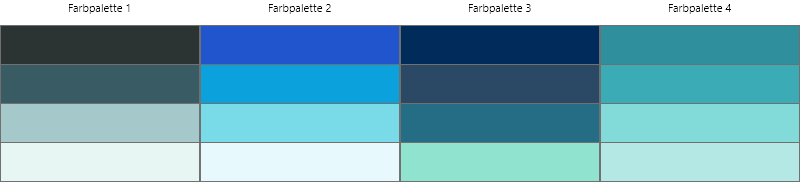
\includegraphics[width=\textwidth]{media/color_palettes}
        \caption{Verschiedene Farbpaletten von Colorhunt}
    \end{figure}

    Als ich die Paletten Timo gezeigt habe, un seine Meinung darüber einzuholen hat er alle nicht wirklich passend
    gefunden. Er hat mir noch ein weiteres Tool gezeigt, welche für Farbpaletten genutzt werden kann. Zudem hat er
    mir direkt eine Farbpalette gezeigt, welche ich für mein Thema verwenden kann. Diese hat auch mich mehr
    angesprochen wie diese Paletten, die ich herausgesucht hatte. Daher habe ich dann auch diese Palette verwendet.
    Aussehen tut die Palette wie folgt:

    \begin{figure}[h]
        
\includegraphics[width=\textwidth]{media/color_palette}
        \caption{Farbpalette von Coolors, welche Timo mir empfohlen hat}
    \end{figure}

    %Kapitel 3.3 - Mockups
    \subsection{Mockups}
    Um die Webseite grob zu designen wollte ich ein Mockup-Programm nutzen. Nachfolgend werde ich Dokumentieren,
    wie ich das Mockup-Programm ausgewählt habe, wie ich die Mockups gestaltet habe und zu guter letzt auch
    die Mockups selbst in die Dokumentation einfügen.

    %Kapitel 3.3.1 - Auswahl des Mockup-Programms
    \subsubsection{Auswahl des Mockup-Programms}
    Um herauszufinden, welches Mockup-Programm ich während des Storyboards und E-Portfolio verwende, habe ich
    mich im Internet informiert, welche verschiedenen Mockup-Programme dass es gibt. Folgende Programme habe
    ich gefunden und genauer analysiert:

    \begin{itemize}
        \item Balsamiq Mockups 3
        \item Moqups.com
        \item Adobe xD
        \item Mockplus.com
    \end{itemize}\\
    Um mich auf ein Tool festzulegen, habe ich Kriterien definiert, und anhand dieser die Tools bewertet. So
    kann ich anschliessend in der Entscheidungsmatrix ablesen, welches Mockup-Programm ich nachher effektiv
    nutze. Folgende Kriterien habe ich vorgängig definiert:

    \begin{itemize}
        \item Erfahrung \textrightarrow Wie viel Erfahrung habe ich bereits mit diesem Tool?
        \item Preis \textrightarrow Wie viel kostet das Tool (je weniger, desto besser)
        \item Funktionalität \textrightarrow Bietet mir das Tool alle Funktionalitäten die ich benötige?
    \end{itemize}
    Um die Entscheidungsmatrix auszufüllen, werde ich eins bis fünf Punkte vergeben. Ein Punkt ist dabei das tiefste
    und fünf das höchste. Das Tool mit den total meisten Punkten gewinnt am Schluss.\\

    \begin{center}
        \begin{tabular}{ | p{4cm} | p{2.5cm} | p{2.5cm} | p{3cm} | p{2.5cm} | }
            \hline
            & \textbf{Erfahrung} & \textbf{Preis} & \textbf{Funktionalität} & \textbf{Total Score} \\ \hline
            \textbf{Balsamiq Mockups} & 3                  & 2              & 4                       & 10                   \\ \hline
            \textbf{Moqups.com}       & 1                  & 2              & 3                       & 6                    \\ \hline
            \textbf{Adobe xD}         & 5                  & 4              & 5                       & 14                   \\ \hline
            \textbf{Mockplus.com}     & 1                  & 3              & 5                       & 9                    \\ \hline
        \end{tabular}
    \end{center}
    \\
    \textbf{Begründung der Entscheidung}\\
    Anhand der obigen Entscheidungsmatrix habe ich mich für das Programm Adobe xD entschieden. Dies hat mehrere
    Gründe. Einerseits habe ich in vergangenen Projekten bereits mit xD gearbeitet, andererseits bietet es
    mir neben den Mockups auch die Funktionalität, einen Prototyp zu gestalten. Zudem habe ich durch eine
    Adobelizenz der Schule xD bereits lizenziert, was bei allen anderen Programmen nicht der Fall ist.

    %Kapitel 3.3.2 - Design der Mockups
    \subsubsection{Design der Mockups}
    Das Design der Mockups war recht einfach. Ich habe zwischendurch Michael gefragt wie das Mockup aussieht. Er kennt
    sich bereits aus dem Betrieb super mit UI's aus, ich habe da leider wenig Erfahrung.
    \\\\Animationen habe ich im Mockup nicht dargestellt. Auf der Beispiel-Page sollen später Beispiele für Steine
    erscheinen. Dabei möchte ich animieren wie die Steine in der Theorie gespielt werden müssten.
    Das Video werde ich auf der ``How to Play'' Seite einbetten.

    \pagebreak

    \begin{landscape}
        %Kapitel 3.3.3 - Mockups
        \subsubsection{Mockups}

        Alle Mockups und ein Prototyp kann mittels dem folgenden xD Link abgerufen werden: \href{https://xd.adobe.com/view/f4f23c9c-e25a-4ecb-8a2d-38adebf22483-a1a1/?fullscreen}{Adobe Xd Prototyp}

        \noindent
        \begin{minipage}{1.1\textwidth}
            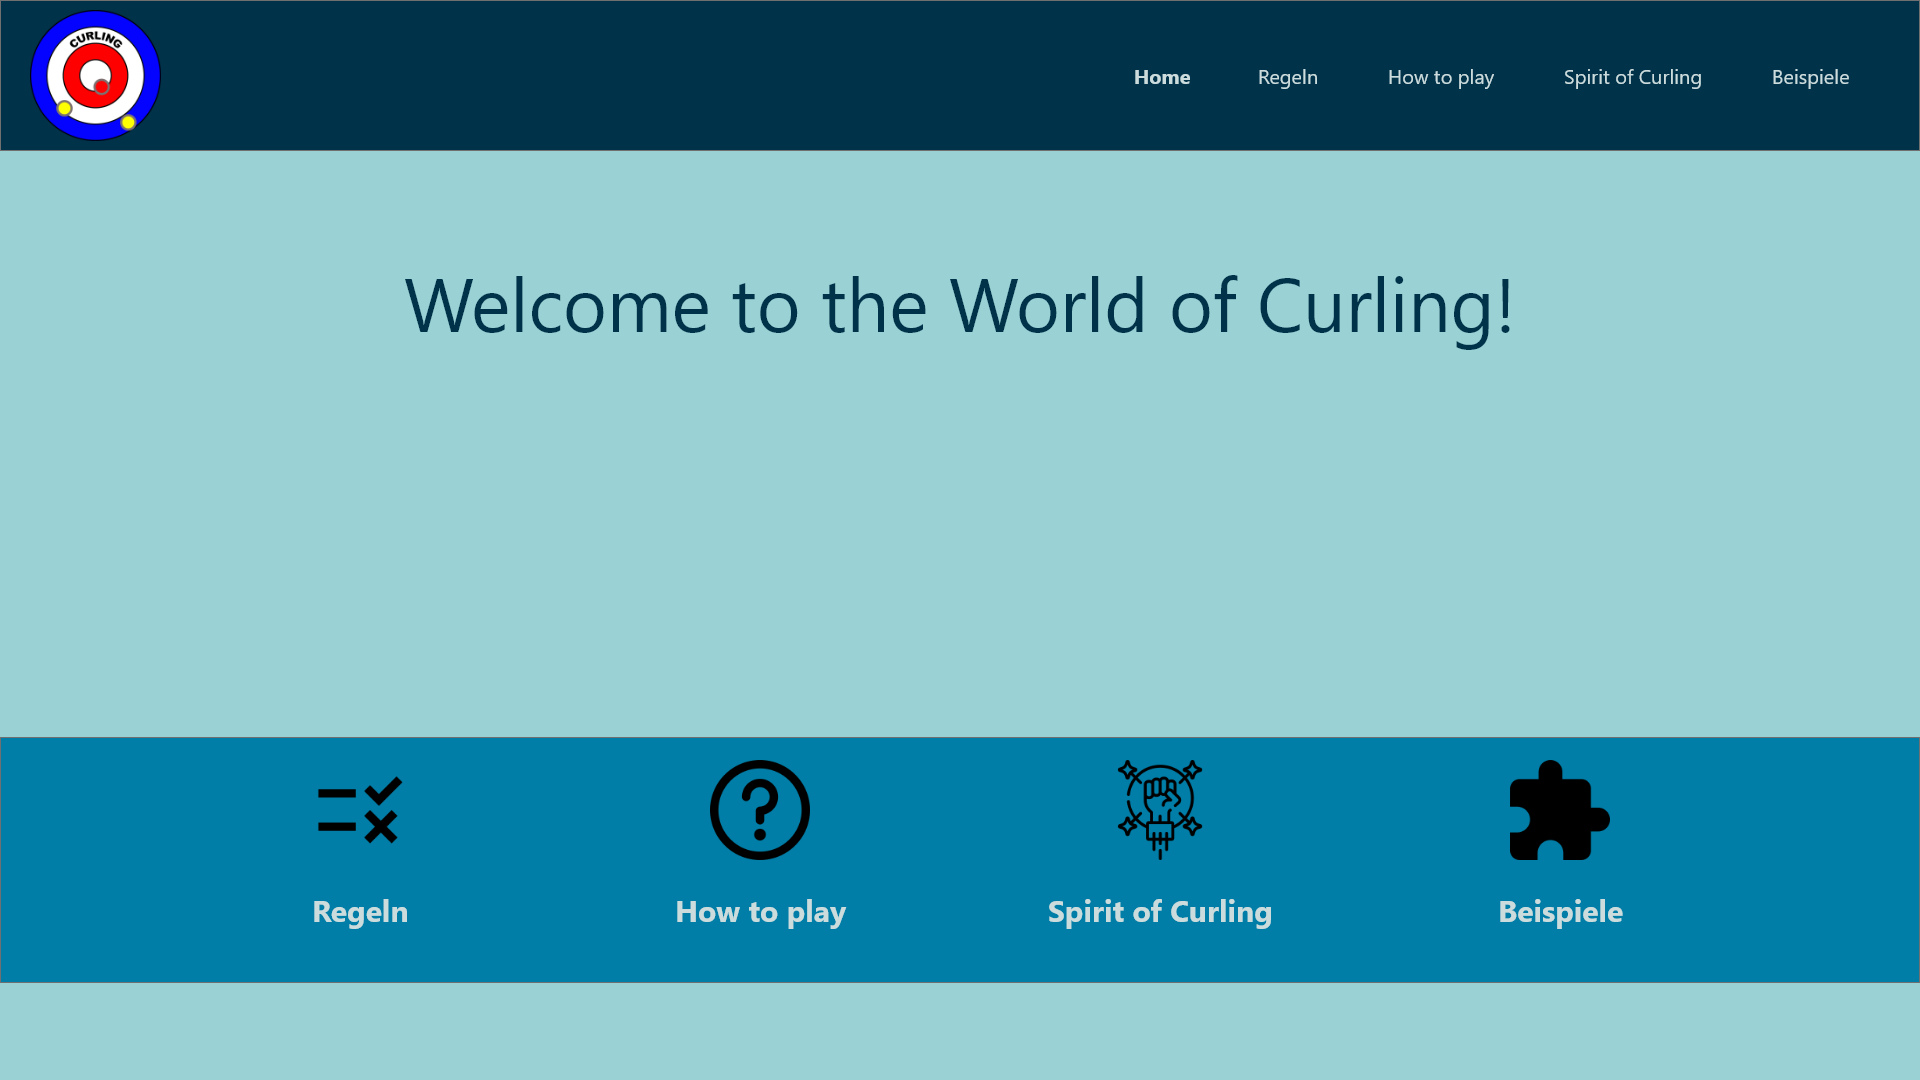
\includegraphics[width=\linewidth]{media/home}
            \captionof{figure}{Startseite}
        \end{minipage}
        \begin{minipage}[c]{0.4\textwidth}
            \raggedleft
            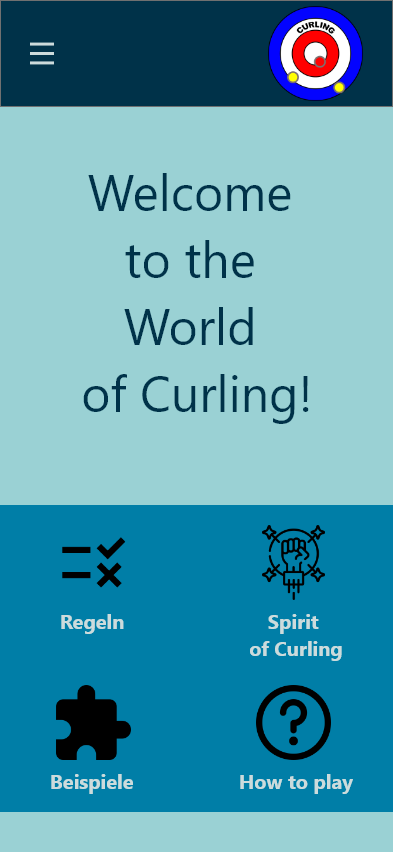
\includegraphics[width=\linewidth]{media/mobile_home}
            \captionof{figure}{Mobile Startseite}
        \end{minipage}
    \end{landscape}
    \pagebreak

    %Kapitel 4 - Bildbearbeitung
    \section{Bildbearbeitung}
    Bei der Bildbearbeitung habe ich mich dazu entschieden, einen simplen schwarz-weiss Filter auf das Bild
    anzuwenden, und einen Teil des Bildes wieder farbig zu machen.\\
    Dafür habe ich GIMP verwendet, welches ein Open-Source Bildeditor ist, welchen wir im Unterricht im Modul
    152 bereits näher kennengelernt haben.


    %Kapitel 4.1 - Bildbearbeitungsmethode
    \subsection{Bildbearbeitungsmethode}
    Ich habe mich für ein Foto aus der Vogelperspektive entschieden, da ich nur so die gesamte Spielfläche
    auf das Bild bekomme. Fotografiert habe ich dieses mit einer Drohne, da ich andere Kameras nicht so hoch
    über das Eis bekomme. Das unbearbeitete Foto sieht dann wie folgt aus:\\
    \begin{figure}[h]
        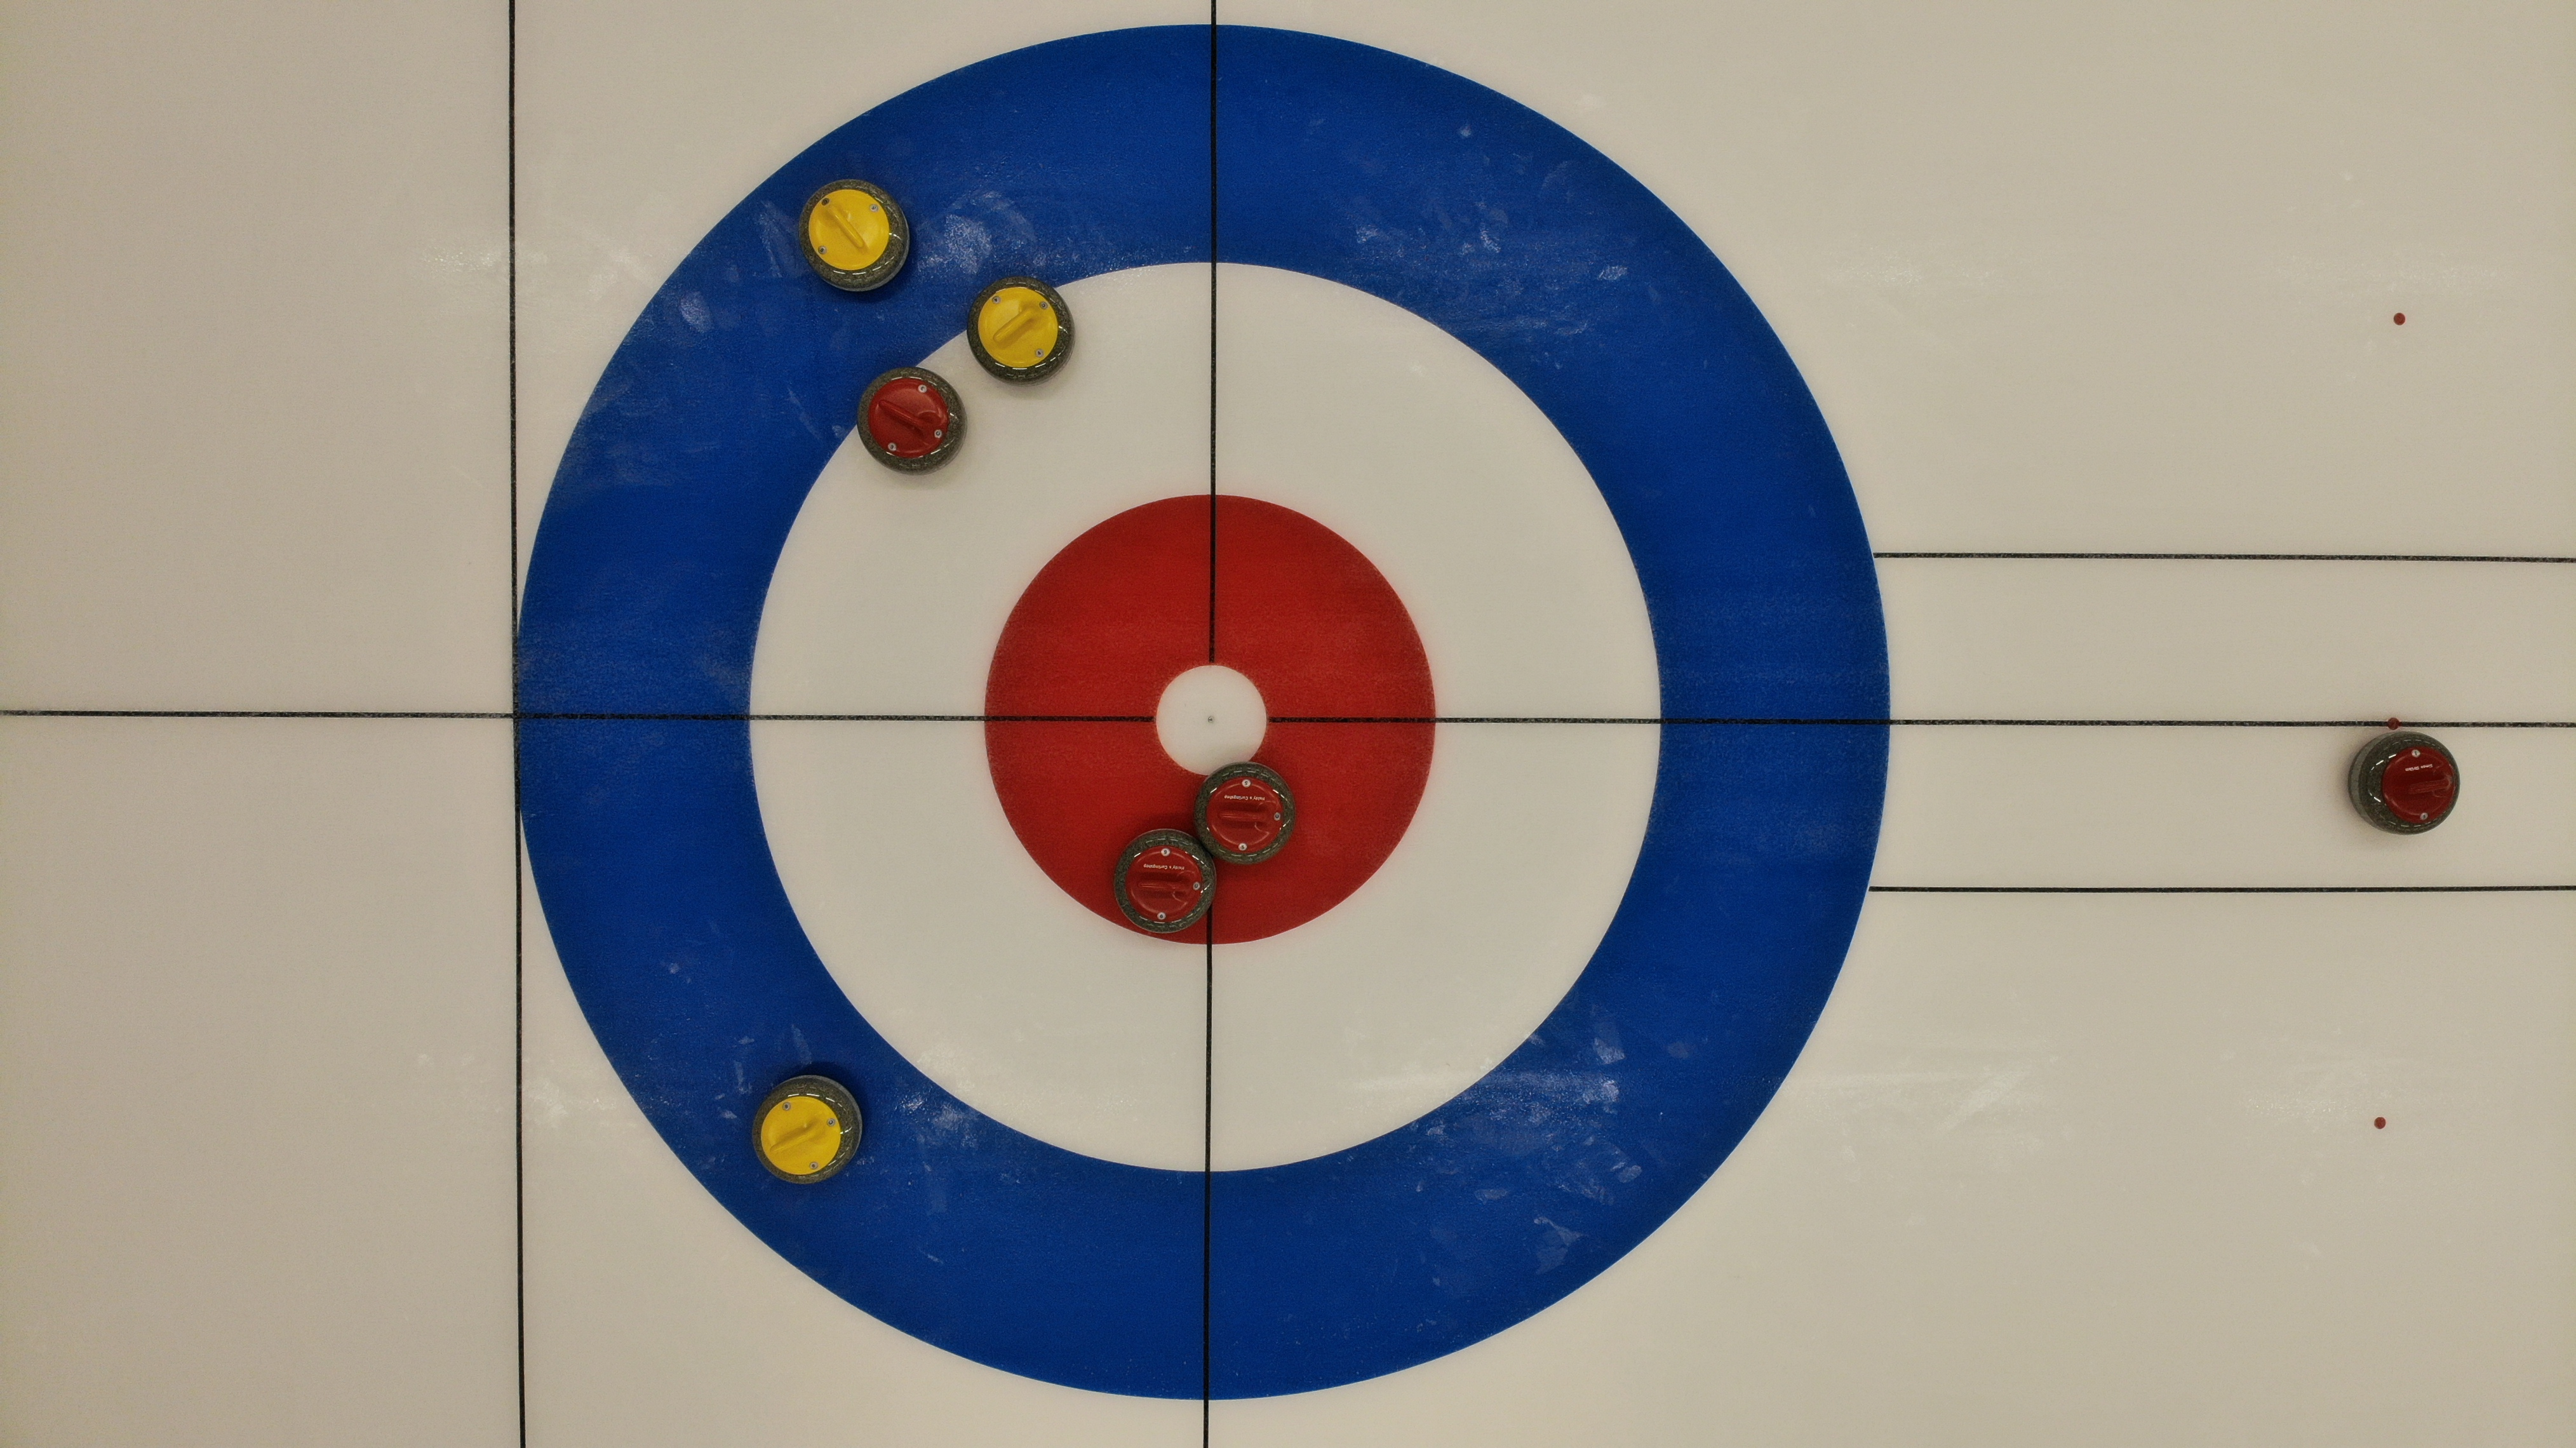
\includegraphics[width=\textwidth]{media/unedited}
        \caption{Bild eines Curling-Hauses ohne Bearbeitung}
    \end{figure}

    \pagebreak

    \textbf{Anleitung zur Bildbearbeitung}\\
    Im folgenden werde ich Schritt für Schritt erklären, wie ich das Bild bearbeitet habe.

    \begin{enumerate}
        \item Bild in GIMP importieren
        \item In der Ebenenauswahl (standardmässig unten rechts) die aktuelle Ebene auswählen und mit rechts-klick
        anwählen. Dort dann ``Ebene duplizieren'' anklicken.
        \item Einer der Layer muss nun Schwarz-Weiss gefärbt werden. Dies kann unter ``Farben'' und dann
        ``Entsättigen'' gemacht werden.

        \begin{figure}[h]
            \centering
            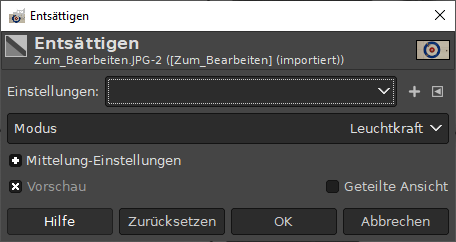
\includegraphics[height=4cm]{media/menu_desaturate}
            \caption{Dialog zum Entsättigen einer Ebene (Schritt 3)}
        \end{figure}

        \item Auf dieser Ebene, welche entsättigt wurde und nun schwarz-weiss ist, wenden wir nun eine
        Ebenenmaske an. Diese ist dafür da, dass wir anschliessend die Transparenz dieses Layers bearbeiten können.
        Die Ebenenmaske kann in der Ebenenauswahl hinzugefügt werden. Dazu die entsprechende Ebene rechtsklicken und
        anschliessend die Option ``Ebenenmaske hinzufügen'' auswählen. Im Dialog habe ich ausgewählt, dass eine weisse
        Ebenenmaske hinzugefügt wird.

        \begin{figure}[h]
            \centering
            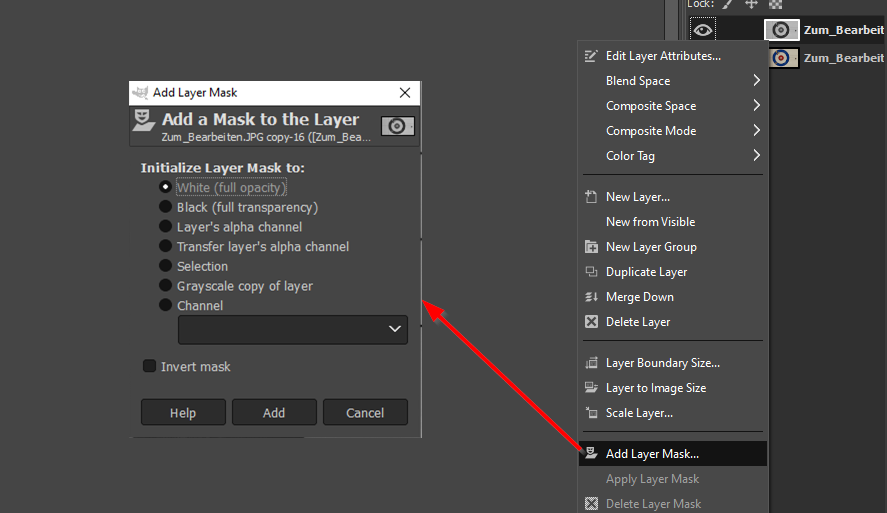
\includegraphics[height=8cm]{media/layer_mask}
            \caption{Dialog zum hinzufügen der Ebenenmaske}
        \end{figure}

        \item Das Pinselwerkzeug auswählen und auf eine brauchbare Grösse einstellen. Wichtig ist, dass ein zu grosser
        Pinsel auch wieder zu viel Farbe aufdeckt.
        \item Mit dem Pinselwerkzeug und gedrückter linker Maustaste diese Bereiche überfahren, welche wieder
        farbig sein sollten.
    \end{enumerate}

    \pagebreak
    Das fertige Bild sieht dann wie folgt aus:\\

    \begin{figure}[h]
        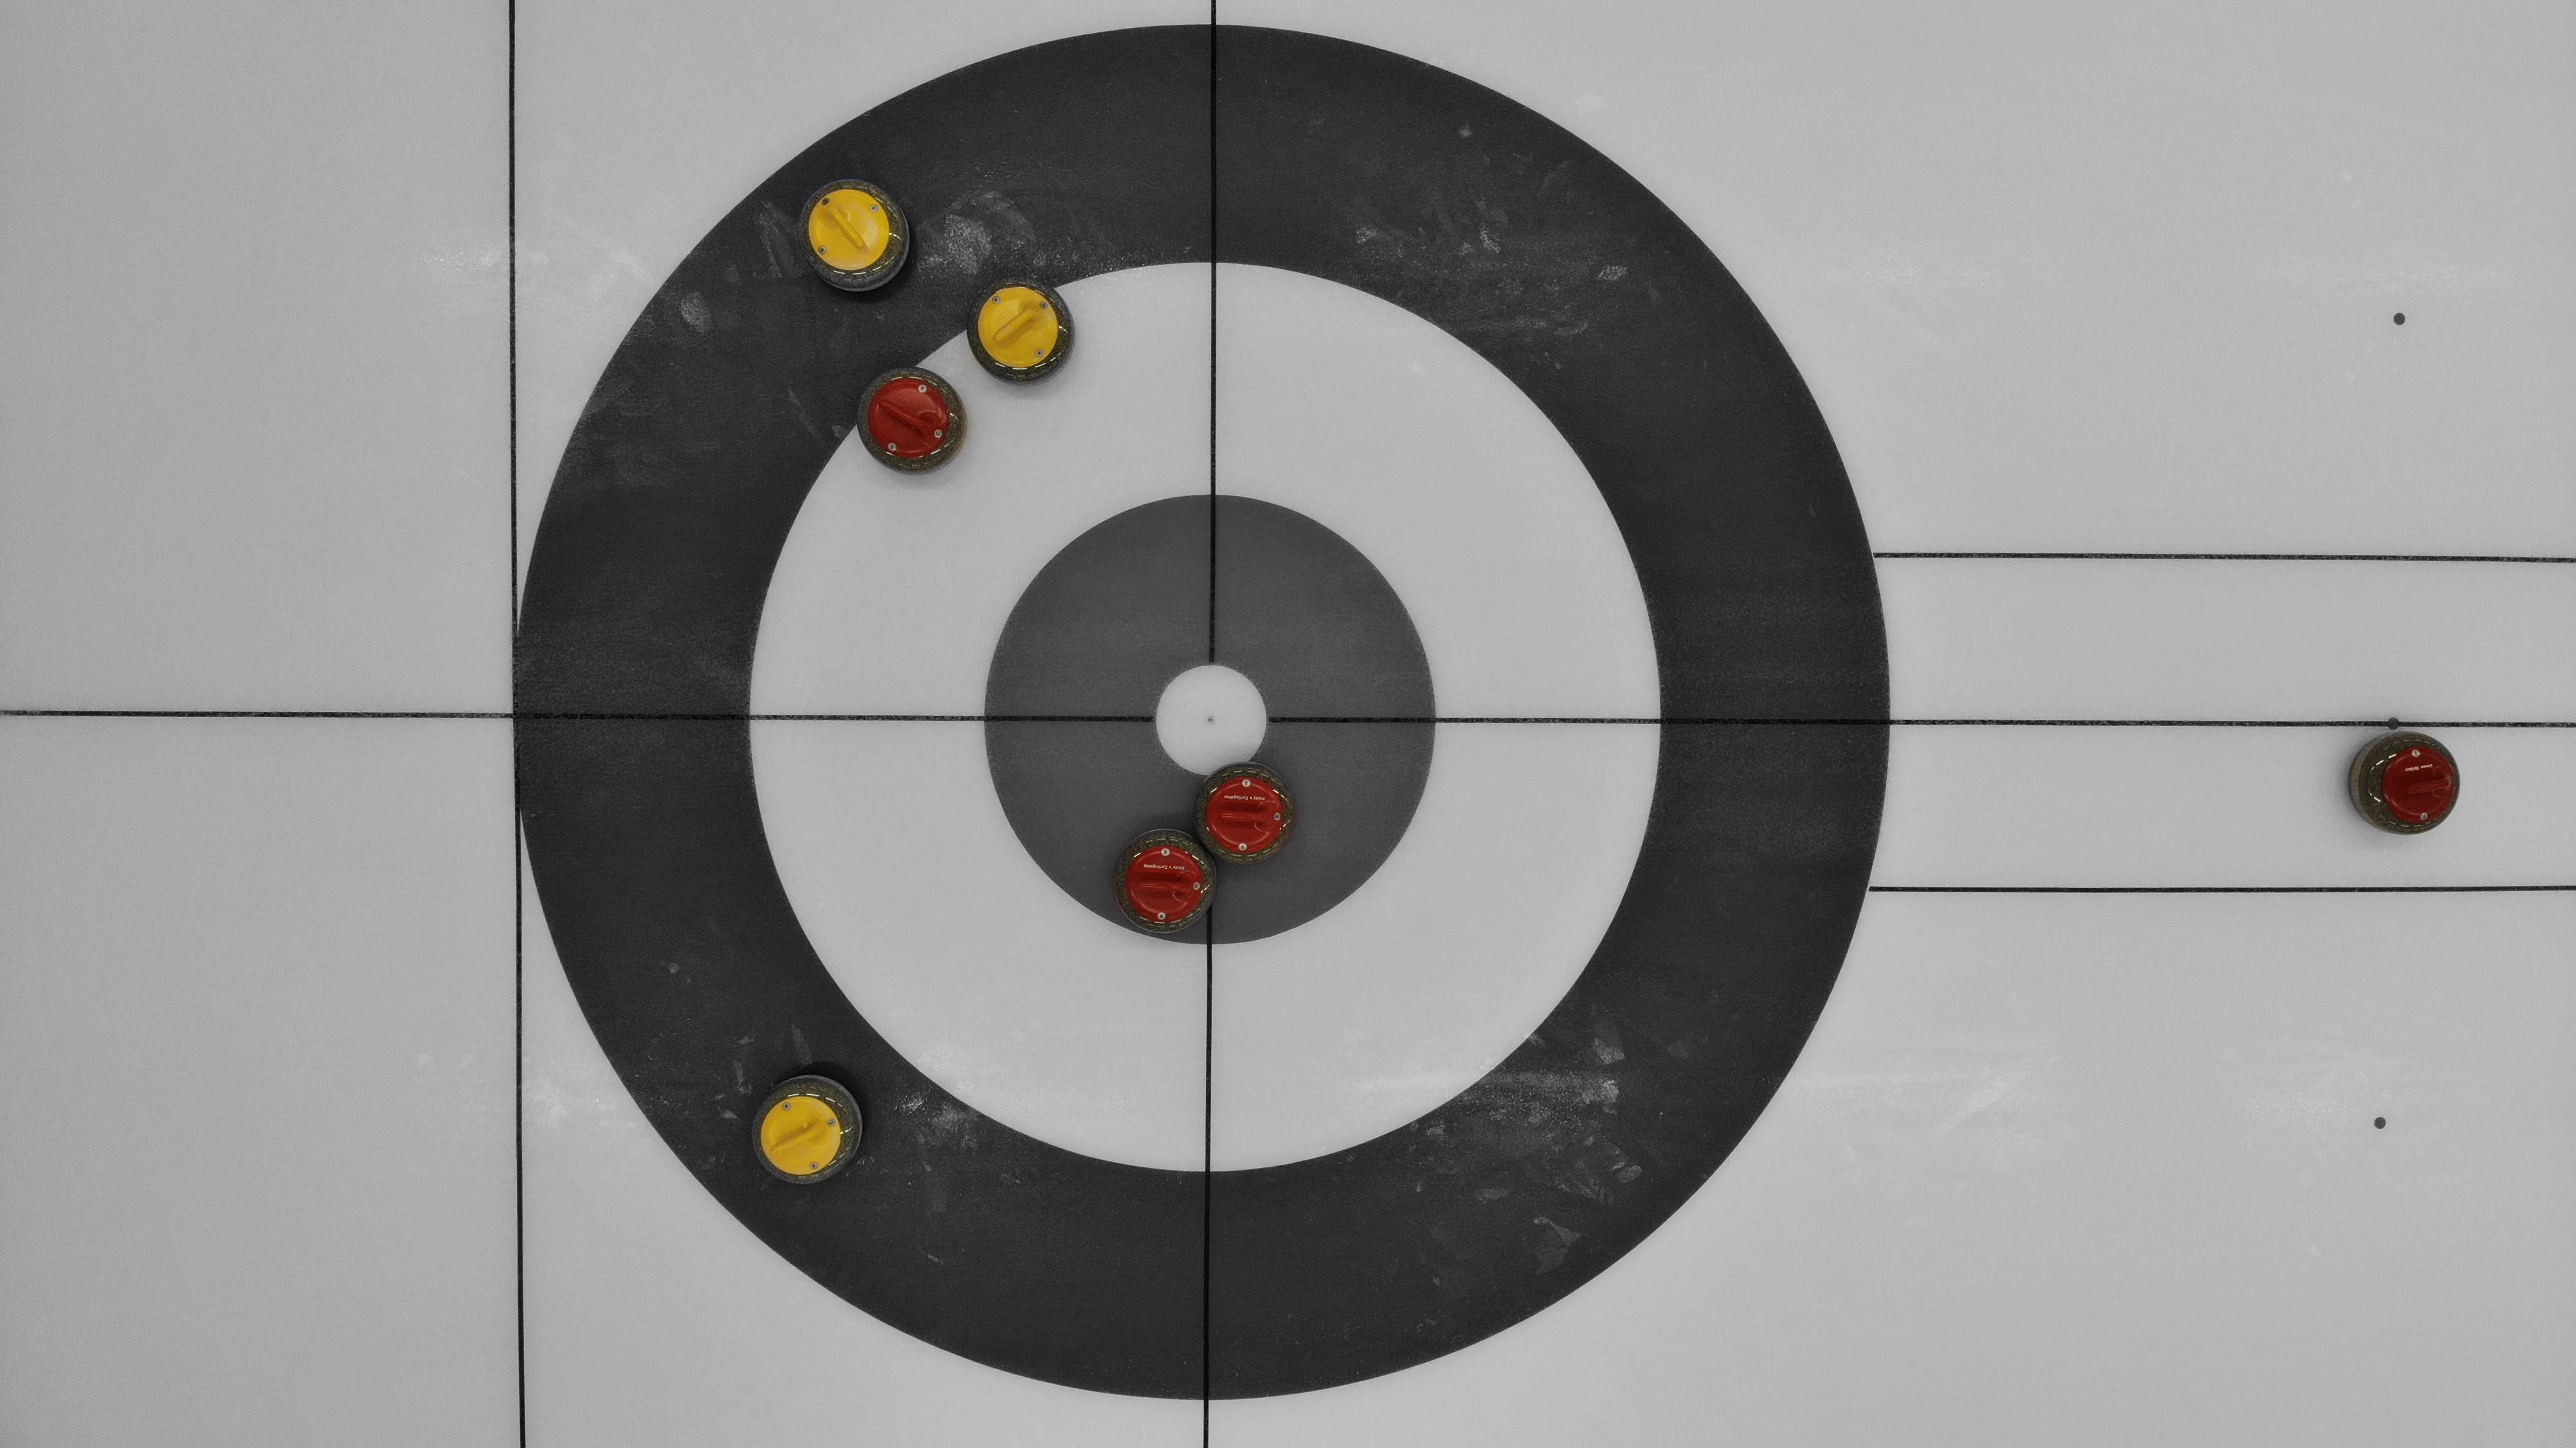
\includegraphics[width=\textwidth]{media/edited}
        \caption{Bild eines Curling-Hauses mit Schwarz-Weiss Filter über allem, ausser den Steinen}
    \end{figure}


    %Kapitel 5 - Logo
    \section{Logo}
    Zu einem E-Portfolio gehört natürlich auch ein passendes Logo. In den folgenden Kapiteln werde ich erläutern, was
    die Idee hinter dem Logo ist, wie das Logo designt wurde und wie das Logo aussieht.

    %Kapitel 5.1 - Idee
    \subsection{Idee}
    Die Idee hinter dem Logo ist eigentlich recht simpel. Das Logo soll den Curling-Sport auf einen Blick zeigen. Ich
    persönlich habe dabei an das Curling Haus gedacht, also der Teil des Spielfeldes, in den die Steine gespielt werden.
    Um diesen Ort dreht sich das ganze Spiel. Da auf den sogenannten Rinks (die einzelnen Bahnen) auch oft Werbung in
    das Eis eingelassen sind, habe ich so den Schriftzug ``Curling'' integriert.

    \noindent\begin{minipage}{0.6\textwidth}
                         %Kapitel 5.2 - Erstellung des Logos
                 \subsection{Erstellung des Logos}
                 Begonnen habe ich das Logo in Adobe xD. Dort hatte ich bereits die einzelnen Ringe des Hauses gezeichnet.
                 Diese dienen während dem Spiel der einfacheren Bestimmung der Entfernung der Steine. Diese haben
                 möglichst unterschiedliche Farben, dass die einzelnen Ringe eifach voneinander unterscheidbar sind.
                 Dies habe ich hier realitästsgetreu nachgefärbt. Nach dem Zeichnen und färben der Ringe hat das Logo
                 wie rechts ersichtlich ausgsesehen.
    \end{minipage}
    \hfill
    \begin{minipage}[c]{0.3\textwidth}
        \raggedleft
        
\includegraphics[width=\linewidth]{media/curling_logo_step1}
        \captionof{figure}{Logo mit den eingefärbten Ringen des Hauses}
    \end{minipage}

    \noindent\begin{minipage}{0.6\textwidth}
                 Die Curlingsteine sind ebenso simpel wie das Haus. Die Steine sind einzelne kleine Kreise aus xD, welche
                 ich so gefärbt habe, dass sie den Farben des Curlings entsprechen. Bei einem richtigen Curlingstein ist
                 von oben einerseits der farbige Plastikgriff (Fachbegriff ``Handle'') sichtbar, aber auch der Stein
                 selbst zu sehen. Dies habe ich damit reproduziert, dass ich in xD die Rahmen des Kreises so skaliert
                 habe, dass sie ungefähr dem reellen Verhältnis entsprachen. Die drei Steine, welche ich anschliessend
                 irgendwo auf dem Haus plaziert habe, sind nun rechts ersichtlich.
    \end{minipage}
    \hfill
    \begin{minipage}[c]{0.3\textwidth}
        \raggedleft
        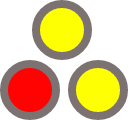
\includegraphics[width=\linewidth]{media/curling_stones}
        \captionof{figure}{Curlingsteine}
    \end{minipage}
    \\\\\\Um nun wie geplant den Schriftzug ``Curling'' in das Haus einzubetten, habe ich GIMP verwendet, da ich zu xD keine
    Anleitung gefunden habe, welche für mich funktioniert hat, um Text an einer Rundung zu biegen. Den bisherigen
    Fortschritt habe ich also als SVG aus Adobe xD exportiert, und in GIMP wieder geöffnet.
    Dort habe ich dann wie folgt die Schrift hinzugefügt:

    \begin{enumerate}
        \item Text ``Curling'' geschrieben
        \item Eine neue Transparente Ebene erstellen
        \item Auf dieser Transparenten Ebene mit dem ``elliptischen Auswahlwerkzeug'' genau den roten Kreis ausgewählt,
        damit der Text später im weissen Kreis steht.
        \item Im Kontextmenü ``Auswahl'' den Punkt ``Nach Pfad'' anklicken. So wird ein Pfad erstellt, entlang dessen
        der Text später stehen wird.
        \item Auf die Ebene mit dem Text zurück und dann mit Rechtsklick auf der Ebene den Punkt ``Text dem Pfad entlang''
        auswählen. So wird der Text dem vorher erstellten Pfad entlang geschrieben.
        \item Als nächsten Schritt wählt man wieder die transparente Ebene aus und drückt Ctrl + Alt + A, um die Auswahl
        verschwinden zu lassen. Dann im Kontextmenü ``Auswahl'' den Punkt ``Nach Pfad'' auswählen.
        \item Dann mit dem Füllwerkzeug den aktuell noch gestrichelten Text in der gewünschten Farbe ausfüllen.
        \item Oben rechts gibt es einen Reiter ``Pfade''. Dort blendet man den Pfad dann mittels dem Auge aus.

        \begin{figure}[h]
            \centering
            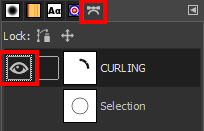
\includegraphics{media/paths}
            \caption{Reiter um Pfade ein- und auszublenden}
        \end{figure}

        \item In der Ebenenauswahl haben wir nun die transparente Ebene mit dem gebogenen Text, den originalen Text,
        und in meinem Fall habe ich noch eine dritte Ebene mit dem bisherigen Fortschritt aus xD.
        \item Nun kann ich den Originalen Text löschen, und den Transparenten Text mit dem Dreh- und Verschiebewerkzeug
        so drehen und verschieben, dass er für mich passt.
    \end{enumerate}

    %Kapitel 5.3 - Fertiges Logo
    \subsection{Fertiges Logo}
    Aus GIMP wieder exportiert sah das fertige Logo wie folgt aus:

    \begin{figure}[h]
        
\includegraphics[width=\textwidth]{media/curling_logo}
        \caption{Fertiges Logo des E-Portfolios}
    \end{figure}

    \pagebreak

    %Kapitel 6 - Technisches Konzept E-Portfolio
    \section{Technisches Konzept E-Portfolio}
    Da ich mich nicht sehr gut mit Webentwicklung auskenne, möchte ich hier gar nicht zu sehr ins Detail gehen.
    Mein E-Portfolio werde ich aus ganz normalem HTML und CSS zusammenbauen. Evtl. wird JavaScript zum Einsatz kommen,
    darauf möchte ich mich aber noch nicht festlegen.
    Für die Bilder möchte ich ein Tool nutzen, welches uns Oliver im Unterricht gezeigt hat. Das Tool heisst Cloudinary,
    und ist dazu da, Bilder automatisch für das Endgerät zu optimieren und optimal zu skalieren. Damit spare ich mir
    nicht nur Speicherplatz auf dem Webserver, sondern habe auch automatisch immer das optimal-grosse Bild.

    %Kapitel 7 - Reflexion
    \section{Reflexion}

    %Kapitel 7.1 - Bildbearbeitung
    \subsection{Bildbearbeitung}
    %TODO text

    %Kapitel 7.2 - Logodesign
    \subsection{Logodesign}
    %TODO text

    %Kapitel 8 - Abbildungsverzeichnis
    \section{Abbildungsverzeichnis}
    \begin{appendix}
        \listoffigures
    \end{appendix}

\end{document}